\documentclass[a4paper,12pt]{article}

\usepackage{rotating}
\usepackage[top=1in, bottom=1in, left=0.75in, right=0.75in]{geometry}
\usepackage{graphicx}
\usepackage[numbers,square,sort&compress]{natbib}
\usepackage{setspace}
\usepackage[cdot,mediumqspace,]{SIunits}
\usepackage{caption}
\usepackage{subcaption}
\usepackage{mathtools}
\usepackage{authblk}
\usepackage{float}
\renewcommand{\thesubsection}{\thesection.\alph{subsection}}
\providecommand{\e}[1]{\ensuremath{\times 10^{#1}}}

\begin{document}
\onehalfspacing
\title{PHY 407 Lab 9}
\author{Natalie Price-Jones, 999091021}
\date{7 November 2014}
\affil{\small{natalie.price.jones@mail.utoronto.ca}}
\maketitle

\section{Question 2}

\begin{figure}[H]
\centering
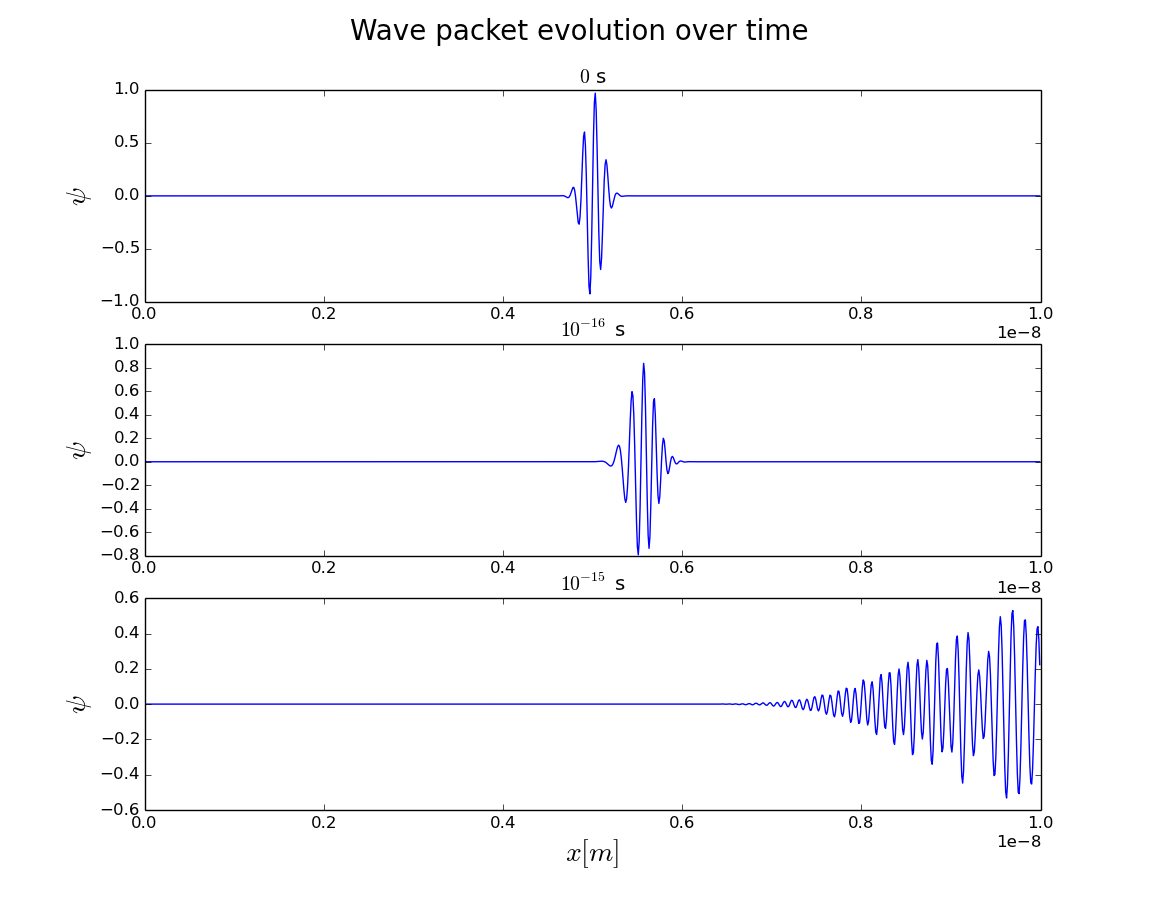
\includegraphics[width = \linewidth]{lab9q2.png}
\caption{}
\label{fig:q2}
\end{figure}

\section{Question 3}

\begin{figure}[H]
\centering
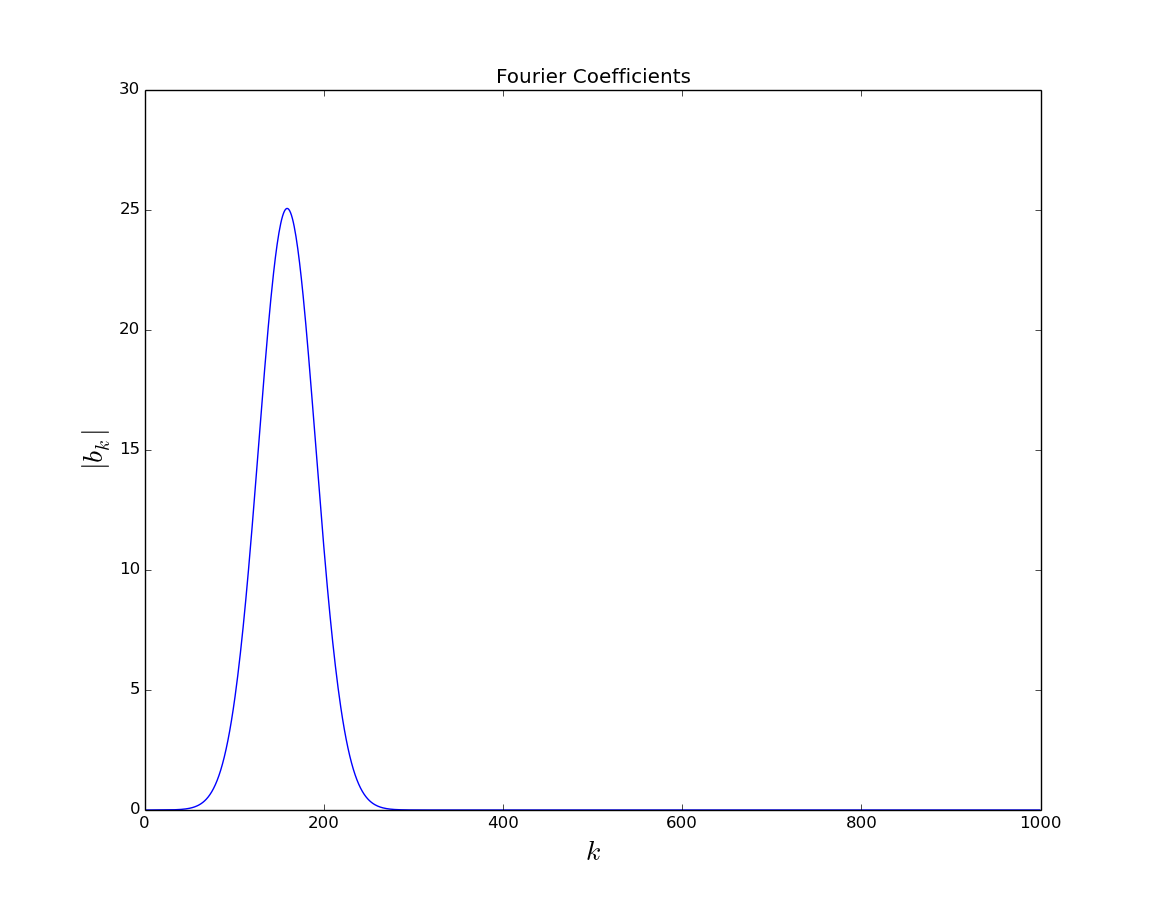
\includegraphics[width = \linewidth]{lab9q3.png}
\caption{}
\label{fig:q3}
\end{figure}

\section{Question 4}

\begin{figure}[H]
\centering
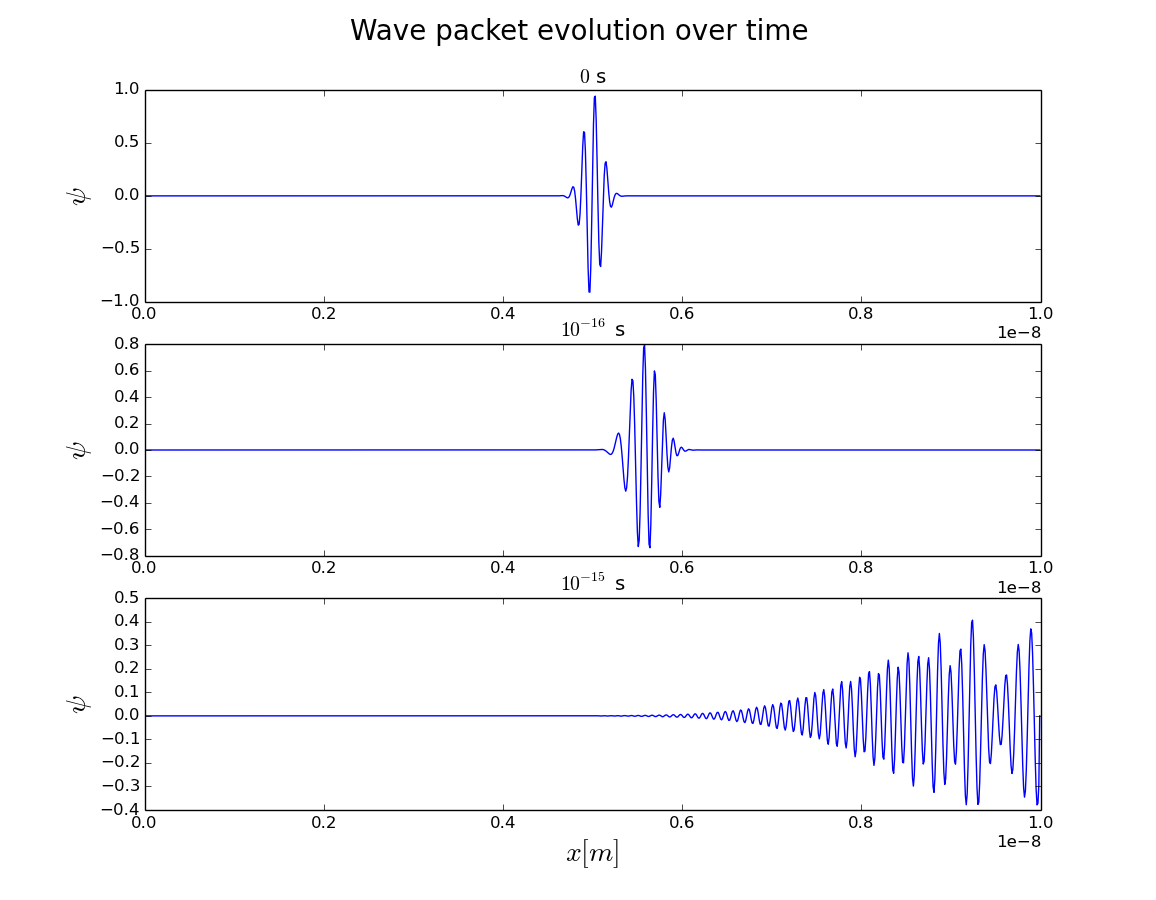
\includegraphics[width = \linewidth]{lab9q4.png}
\caption{}
\label{fig:q4}
\end{figure}

\end{document}